\input{Header-FSM.tex}

\begin{document}

\begin{page}
\centering
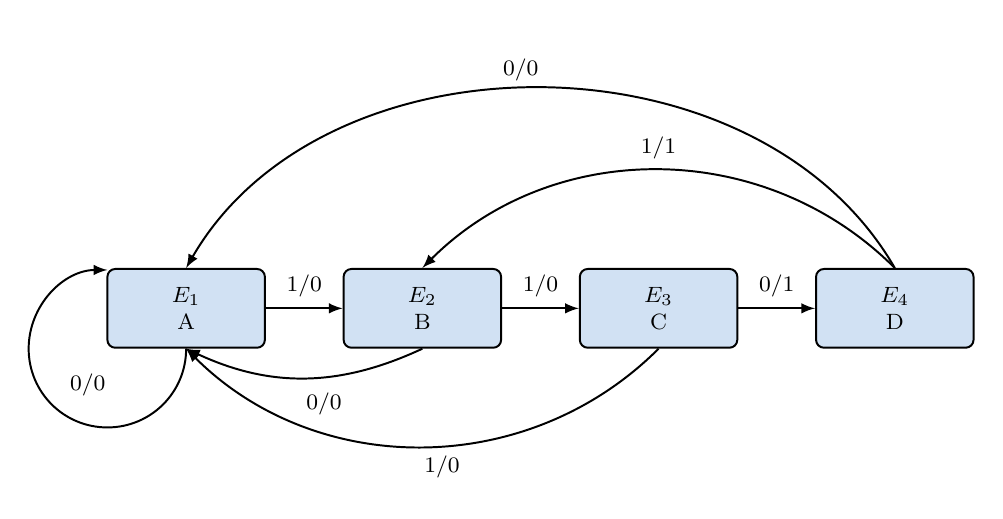
\begin{tikzpicture}

	%DEFINICIONES
	\tikzstyle{every node}=[font=\footnotesize]	
	\tikzstyle{base} = [draw, align=center, line width=0.25mm, fill={rgb,255:red,204; green,255; blue,204}, minimum width=2cm, minimum height=1.25cm]	
	\tikzstyle{blank} = [align=center, inner sep=0pt, outer sep=0pt]	
	\tikzstyle{block} = [draw, rounded corners=0.1cm, align=center, line width=0.25mm, fill={rgb,255:red,209; green,225; blue,243}, minimum width=2cm, minimum height=2cm]	
	\tikzstyle{flecha} = [->, line width=0.25mm, >=latex]
	\tikzstyle{linea} = [line width=0.25mm, >=latex]
	\tikzstyle{meas} = [draw, rectangle, densely dashed, minimum width=0.2cm, minimum height=0.6cm]
	\tikzstyle{circulo} = [circle,fill=black,inner sep=0pt,minimum size=3pt]
	
	%BLOQUES
	\draw(0,0) node[block, minimum height=1cm](1){$E_1$ \\ A};
	\draw(3,0) node[block, minimum height=1cm](2){$E_2$ \\ B};
	\draw(6,0) node[block, minimum height=1cm](3){$E_3$ \\ C};
	\draw(9,0) node[block, minimum height=1cm](4){$E_4$ \\ D};
	
	%FLECHAS
	\draw [flecha] (1.east) -- (2.west) node[midway, blank, label=above:$1/0$]{};
	\draw [flecha] (2.east) -- (3.west) node[midway, blank, label=above:$1/0$]{};
	\draw [flecha] (3.east) -- (4.west) node[midway, blank, label=above:$0/1$]{};
	
	\draw[flecha] (4.north) to[out=135,in=45] (2.north);
	\draw(6,1.75) node[blank, label=above:$1/1$]{};
	
	\draw[flecha] (4.north) to[out=120,in=60] (1.north);
	\draw(4.25,2.75) node[blank, label=above:$0/0$]{};
	
	\draw [flecha] (3.south) to[out=-135,in=-45] (1.south);
	\draw(3.25,-2.3) node[blank, label=above:$1/0$]{};
	
	\draw [flecha] (2.south) to[out=-155,in=-25] (1.south);
	\draw(1.75,-1.5) node[blank, label=above:$0/0$]{};
	
	\draw [flecha] (1.south) to[out=-90,in=0] ++(-1,-1) to[out=180,in=-90] ++(-1,1) to[out=90,in=-180] ++(1,1);
	\draw(-1.25,-1.25) node[blank, label=above:$0/0$]{};
\end{tikzpicture}	
\end{page}

\end{document}